\chapter{Theory}
\label{chapter:theory}

The relevant literature and theories are organised into two sections: barriers and supporting factors of sharing data. The barriers utilize literature from informatics in supply chains, knowledge sharing and institutional theory. The supporting factors consider existing models where data sharing has been enabled, or models that plan such activies in terms of roles, processes, ..

\subsection{Barriers in sharing inter-enterprise data}

The theoretical background for inter-enterprise data sharing is comprised of literature on inter-enterprise knowledge sharing, supply chains,  

The barriers




Sharing data between operators in a single supply chain is a widely studied subject in academia, with researchers pondering on topics such as barriers to information sharing \cite{khurana2011barriers}, global knowledge sharing \cite{myers2008sharing} and information sharing \cite{lee2000information}. Khurana et al. divide barriers to information sharing into six different categories: managerial, organizational, individual, financial, social and cultural. Crucial barriers identified are the financial, technological and organizational barriers for integration of information sharing with supply chain. The barrier with the highest importance is financial constraint for high cost of maintenance, followed by data and information security. The following figure lists identified barriers by category.

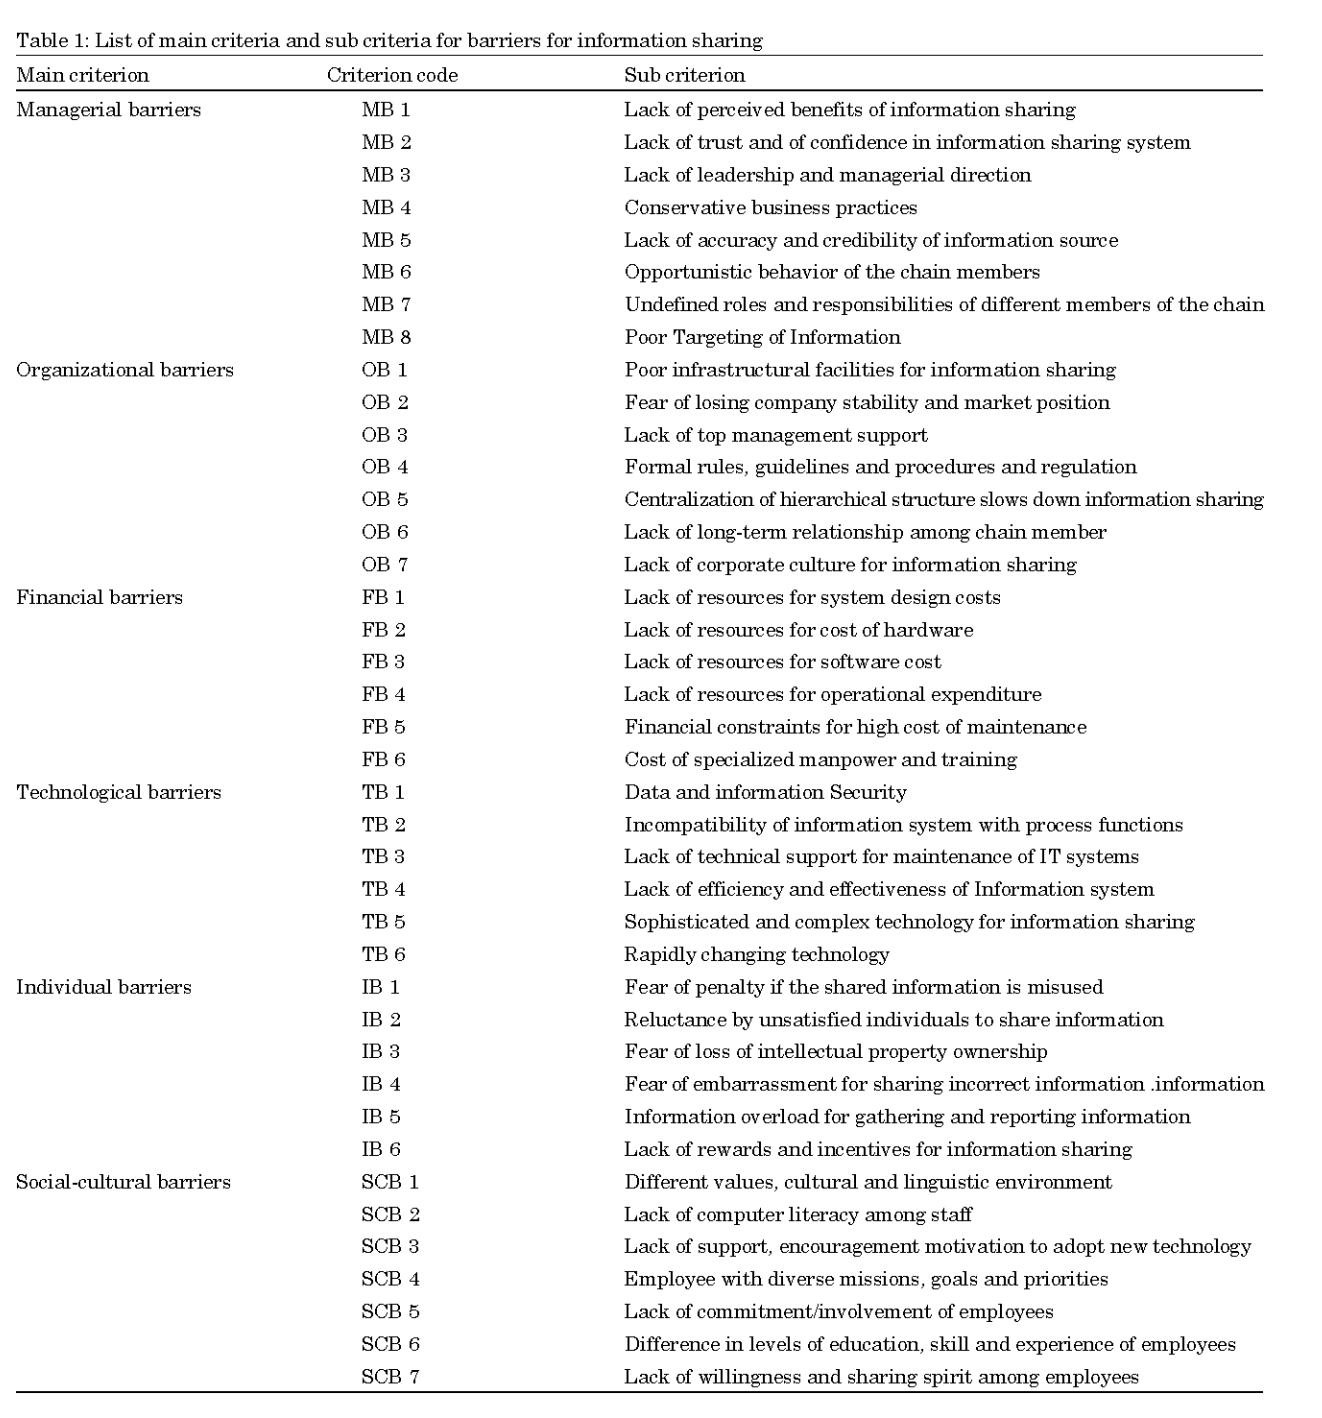
\includegraphics{images/barriers}

Loebecke et al. have studied the strategic paradox of protecting versus sharing knowledge between organizations \cite{loebbecke2016managing}. The authors propose four configurations of inter-organizational knowledge sharing for managing the paradox. The four configurations are the combinations of two types of knowledge and two modes of knowledge sharing. The types are explicit knowledge, which refers to concepts, information and insights that are specifiable and can be formalized into rules and procedures \cite{walsh1987formalization}, and tacit knowledge, which refers to insights and skills that are embedded in individuals or organizational context. The modes of knowledge sharing are unilateral, that takes the characteristics of one-way traffic, and bilateral, which is reciprocal in nature. 

In bilateral sharing of explicit knowledge, participating companies "face a quid pro quo balancing act of sharing and receiving knowledge", and strive for competitive advantage without diluting their unique resources. Each partner might aim to decrease the amount of value of the information the company shares, while also trying to maximize the value the company receives. The article suggests that companies asking for clarifications and additional contextual information beyond the knowledge sharing covered by the contracts is a way to do this.

In bilateral sharing of tacit knowledge, companies might be tempted to deviate from the initial agreements due to partially conflicting interests. An example is delivering limited and possibly inaccurate information, meanwhile enhancing the reception of valuable knowledge. This causes tension in relationships, and potentially escalates uncertainty and distrust \cite{hsu2014examining}. Another issue is managing the coordination between organizations, and preventing individuals from leaking private information into the public domain. 








%Barriers to Information Sharing in Supply Chain of Manufacturing Industries

%http://docsdrive.com/pdfs/academicjournals/ijmsaj/0000/28376-28376.pdf

managerial: 
"do not realize the benefits of information sharing "
"do not have confidence in information sharing system"
"lack of training and experience and low literacy about new technology"

<kuva>





Co-opetition and knowledge transfer %http://ejournal.narotama.ac.id/files/set7.pdf
-



Managing inter-organizational knowledge sharing



chiu2006understanding
%https://www.researchgate.net/profile/Eric_Wang25/publication/222422090_Understanding_knowledge_sharing_in_virtual_communities_An_integration_of_social_capital_and_social_cognitive_theories/links/549ab2060cf2b8037136f46d.pdf

%file:///Users/oris/Downloads/main.pdf
%loebbecke2016managing


\subsubsection{Institutional Theory}
https://www.researchgate.net/publication/265348080_Institutional_Theory_Contributing_to_a_Theoretical_Research_Program




%\subsection{Coopetition}
%http://www.icesi.edu.co/blogs/logisticawww122/files/2012/10/6-Co-opetition-and-Technological-Innovation-in.pdf


\subsection{Supporting factors for sharing data}

The contents and procedures for knowledge transfer are specified in comprehensive contracts \cite{walsh1987formalization}.  


In inter-organizational tacit knowledge sharing, prior research proposes group modes of coordinating work \cite{van1976determinants}. 
%file:///Users/oris/Downloads/main%20(1).pdf


Role concept: https://www.fraunhofer.de/content/dam/zv/en/fields-of-research/industrial-data-space/whitepaper-industrial-data-space-eng.pdf
Data provider
Data user

\subsubsection{Data Governance}
Data governance is a set of practices that ensures data assets are managed comprehensively within an organization. 

%http://cacm.acm.org/magazines/2010/1/55771-designing-data-governance/abstract
Difference between governance and management can be differentiated as follows \cite{khatri2010designing}: governance refers to what decisions must be made to ensure effective management and use of IT, and who makes the decisions. Management involves making and implementing decisions. Therefore, governance establishes who in the organization holds decision rights for determining certain standards, and maintenance involves determining the actual metrics employed.

IT assets and and information assets can also be differentiated \cite{khatri2010designing}: IT assets refers to technologies, such as computers and databases, that help support the automation of well-defined tasks. Information assets refer to facts that have value or potential value that are documented. 


Data governance can be divided into nine different management functions\cite{mosley2010dama}: 


\begin{itemize}
	\item Data quality - defining, monitoring and maintaining data integrity, and improving the quality of data.
	\item Data architecture - the overall structure of the data and resources related to it
	\item Data storage and operations - physical data assets storage, deployment and management
	\item Data operations -
	\item Data development
	\item Data security
	\item Data development
	\item Data security
	\item Reference and master data
	\item Data warehousing and business inteligence
	\item Document and content
	\item Meta-data    
\end{itemize}
%https://www.dama.org/sites/default/files/download/DAMA-DMBOK2-Framework-V2-20140317-FINAL.pdf

%data lifecycle management (tiedon jakaminen ajallisesti rajattua, poisto?), data quality, data security and access management (pitää määritellä tarkkaan mitä dataa antaa), data ownership (analytiikan tulokset, aggregaattidata)

Four management functions, namely 

data lifecycle management, 
data quality, 
data security and access management
-ensure approppriate use of data by appropriate stakeholders


%RQ1: Under which cross-licensing models and other commercial conditions should the cross-enterprise data sharing be governed?
data ownership (provenance)
-who are accountable for quality and security of critical data
-what ownership actually means
-define the rights and responsibilities of owners
-indicate whether and how those responsibilities change over time

\subsubsection{Extended Enterprise}
Extended enterprise is a term created by Chrysler, originally used to define businesses with an extended global supply chain of thousands of suppliers and distributors \cite{dyer2000collaborative}. Another definition is "the entire set of collaborating companies both upstream and downstream, from raw materials to end-use consumption, that work together to bring value to the marketplace” \cite{spekman2004risky}. 

The problem areas extended enterprises often deal with consist of business process integrations and time-cost reductions. 

Recently, a knowledge-based view of the extended enterprise model has been created \cite{alguezaui2014knowledge}. This model takes into account recent research in supply-chain management, operations, strategy and innovation. 



\subsubsection{Business models}
New Service-provider and Business-model Disruption in the Industrial Internet of Things (IIoT)
https://www.iiconsortium.org/news/joi-articles/2016-June-New-Service-provider-and-Business-model-Disruption-in-the-Industrial-Internet-of-Things.pdf



%\subsection{Joint ventures}

%"In European law, the term 'joint venture' (or joint undertaking) is an elusive legal concept, better defined under the rules of company law. "




%knowledge-based extended enterprise: https://www.researchgate.net/profile/Raffaele_Filieri/publication/264437079_A_knowledge-based_view_of_the_extending_enterprise_for_enhancing_a_collaborative_innovation_advantage/links/5422bbaf0cf26120b7a3fca6.pdf

	

%strategia & it: http://innovation-regulation2.telecom-paristech.fr/wp-content/uploads/2007/05/DEDM13_Aligning-Alignment-with-Strategic-Context-A-Literature-Review.pdf

%\subsection{Processing industry}

%Teoria
%  -Relevantit prosessiteollisuuden kirjallisuus
%  -miten massiivisessa valmistavassa teollisuudessa voidaan hyödyntää uusia ICT-ratkaisuja?
%  -Operations management, Maintenance operations management, Teollisuustaloudellinen näkökunta, Joint / shared enterprise data, IoT / teknologiakulma